\documentclass[a4paper,10pt, twocolumn]{article}
\usepackage{amsmath}
\usepackage{graphicx}
\usepackage[font={small,it}]{caption}

\begin{document}

\title{Coursework 1: Analysis of visualisations}
\author{Alun Meredith}
\maketitle

\begin{abstract}
When producing there is a lot of conventional logic governing design choices. We explore three visualisations which defy some of these conventions to invoke imagery and produce more eye-catching and memorable graphics and discuss where they succeed and fail, offering improvement suggestions where appropriate. 
\end{abstract}
\section{Pipelines\cite{xkcd}}
\begin{figure}[!b]
	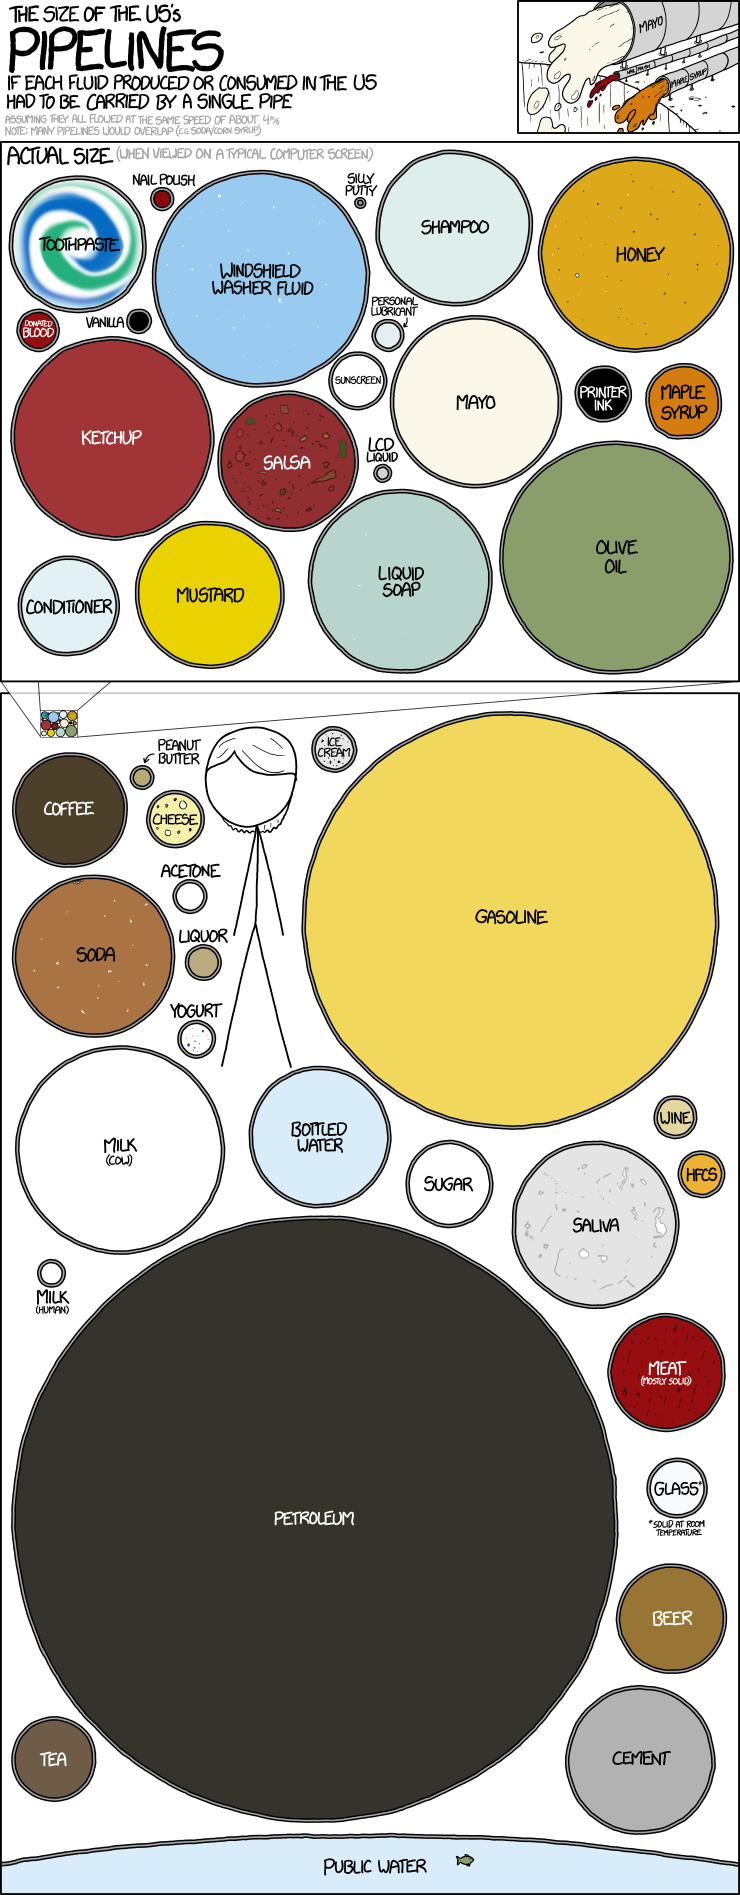
\includegraphics[width=0.3\textwidth]{xkcd.png}
	\centering
	\caption{Volumes of liquids produced and consumed by the US dispalayed as the cross section of the pipe required to transport them at 4 m/s. Source: xkcd.com\cite{xkcd}.}
	\label{fig:xkcd}
\end{figure} 

This figure taken from the popular science/engineering web-comic 'xkcd' visualises the quantities of different liquids produced or consumed by the US. It does so through a scenario where each area is a measure of the volume of liquid flowing through a pipe at a rate of 4 m/s. This allows readers to better conceptualise volumes. 

As a web-comic this exploratory visualisation aims to entertain, intrigue and inform viewers without a specific political message or take away action. The author is trying to allow viewers to perceive the physical volumes of these liquids being consumed/produced as opposed to difficult to conceptualise large numbers in traditional media.  

This concept of visualising volumes of liquid drives many of the design decisions. The choice of chart type, colours, area as the measure, scale and embellishments are all in service to this conceptualisation and helps the audience visualise a volume.  

A categorical variable compared against continuous measure is usually best described by a bar chart\cite{showme} as differences in length are easier to perceive than area \cite{perception}. The author doesn't expect numerical values to be extracted from the areas. Instead comparison is relative. Invoking the imagery, the audience inherently understands area is the scale and the $x^2$ scale also helps to condense the large range of values.  

Some of the colours are indistinguishable as the author plots more than the Kelly's 9 distinguishable colours by colour blind individuals\cite{twentytwo}. However by labelling each circle, including textures and colour choices related to the object being represented the viewer understands each circle represents a different liquid. 

There are however two areas where this visualisation has issues, readability and comprehension. Building on area being hard to interpret the user must extrapolate these into a volume, this makes it difficult for viewers to understand the actual volumes being represented. A reference scale like Olympic swimming pool per second could be added as a to improve volume comprehension.

Similar liquids are not always close together, for example tea and coffee are far apart so more care should taken to ensure liquids users likely compare or similar sizes are close together. The visualisation would benefit from having the data available on mouse-over to facilitate comparisons.   

Finally production and consumption are summarised by this chart making it very difficult to make meaningful conclusions based off this chart. "Design should always support analysis"\cite{tufte} so this should be split into two separate charts provided the data is available. 

\section{Who marries whom\cite{bloomberg}}
 
This figure from the Bloomberg Business website is an interactive visualisation of marriages between professions. It follows a common trope of interactive visualisations which fall away from standard methods of visualising data in order to be unique. 

\begin{figure}[b]
	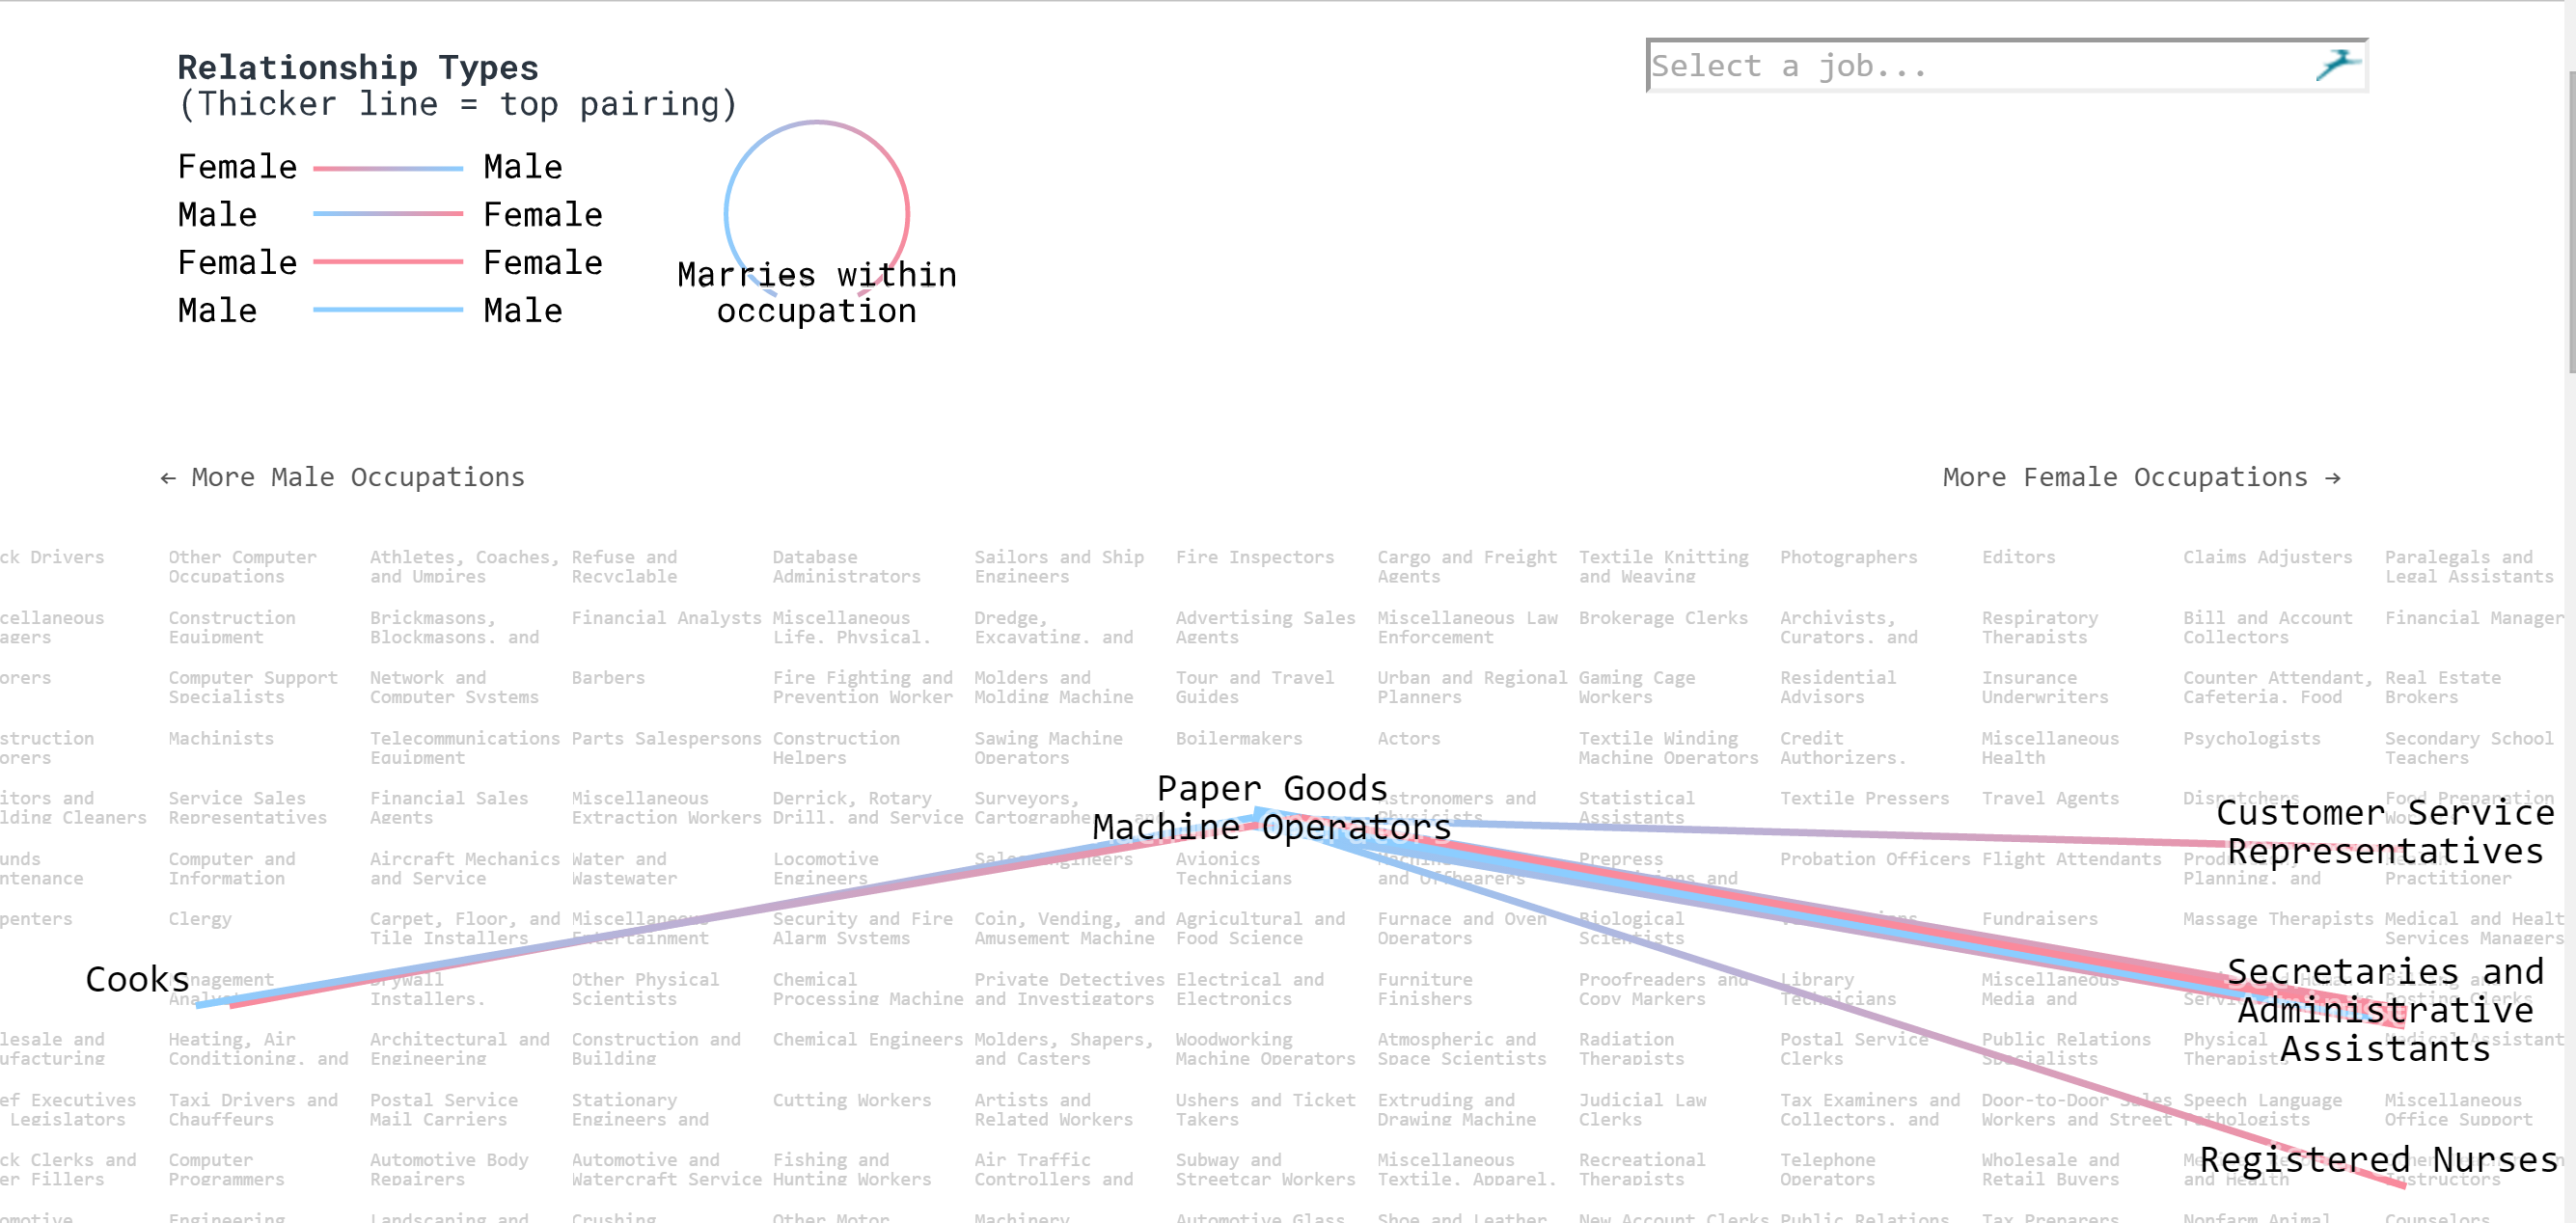
\includegraphics[width=\linewidth]{Bloomberg1.png}
	\centering
	\caption{"This Chart Shows Who Marries CEOs, Doctors, Chefs and Janitors". Chart showing the most common network of marriages between different professions from the 2014 US census. Source: Bloomberg.com \cite{bloomberg}}
	\label{fig:bloomberg}
\end{figure}

Although Bloomberg's website is primarily aimed at business topics it often includes mass media content, the audience is therefore a mass audience with no assumed prior knowledge of statistics. As an exploratory visualisation it's purpose is to use to allow users to explore the data and find patterns. 

\begin{figure}[htbp]
	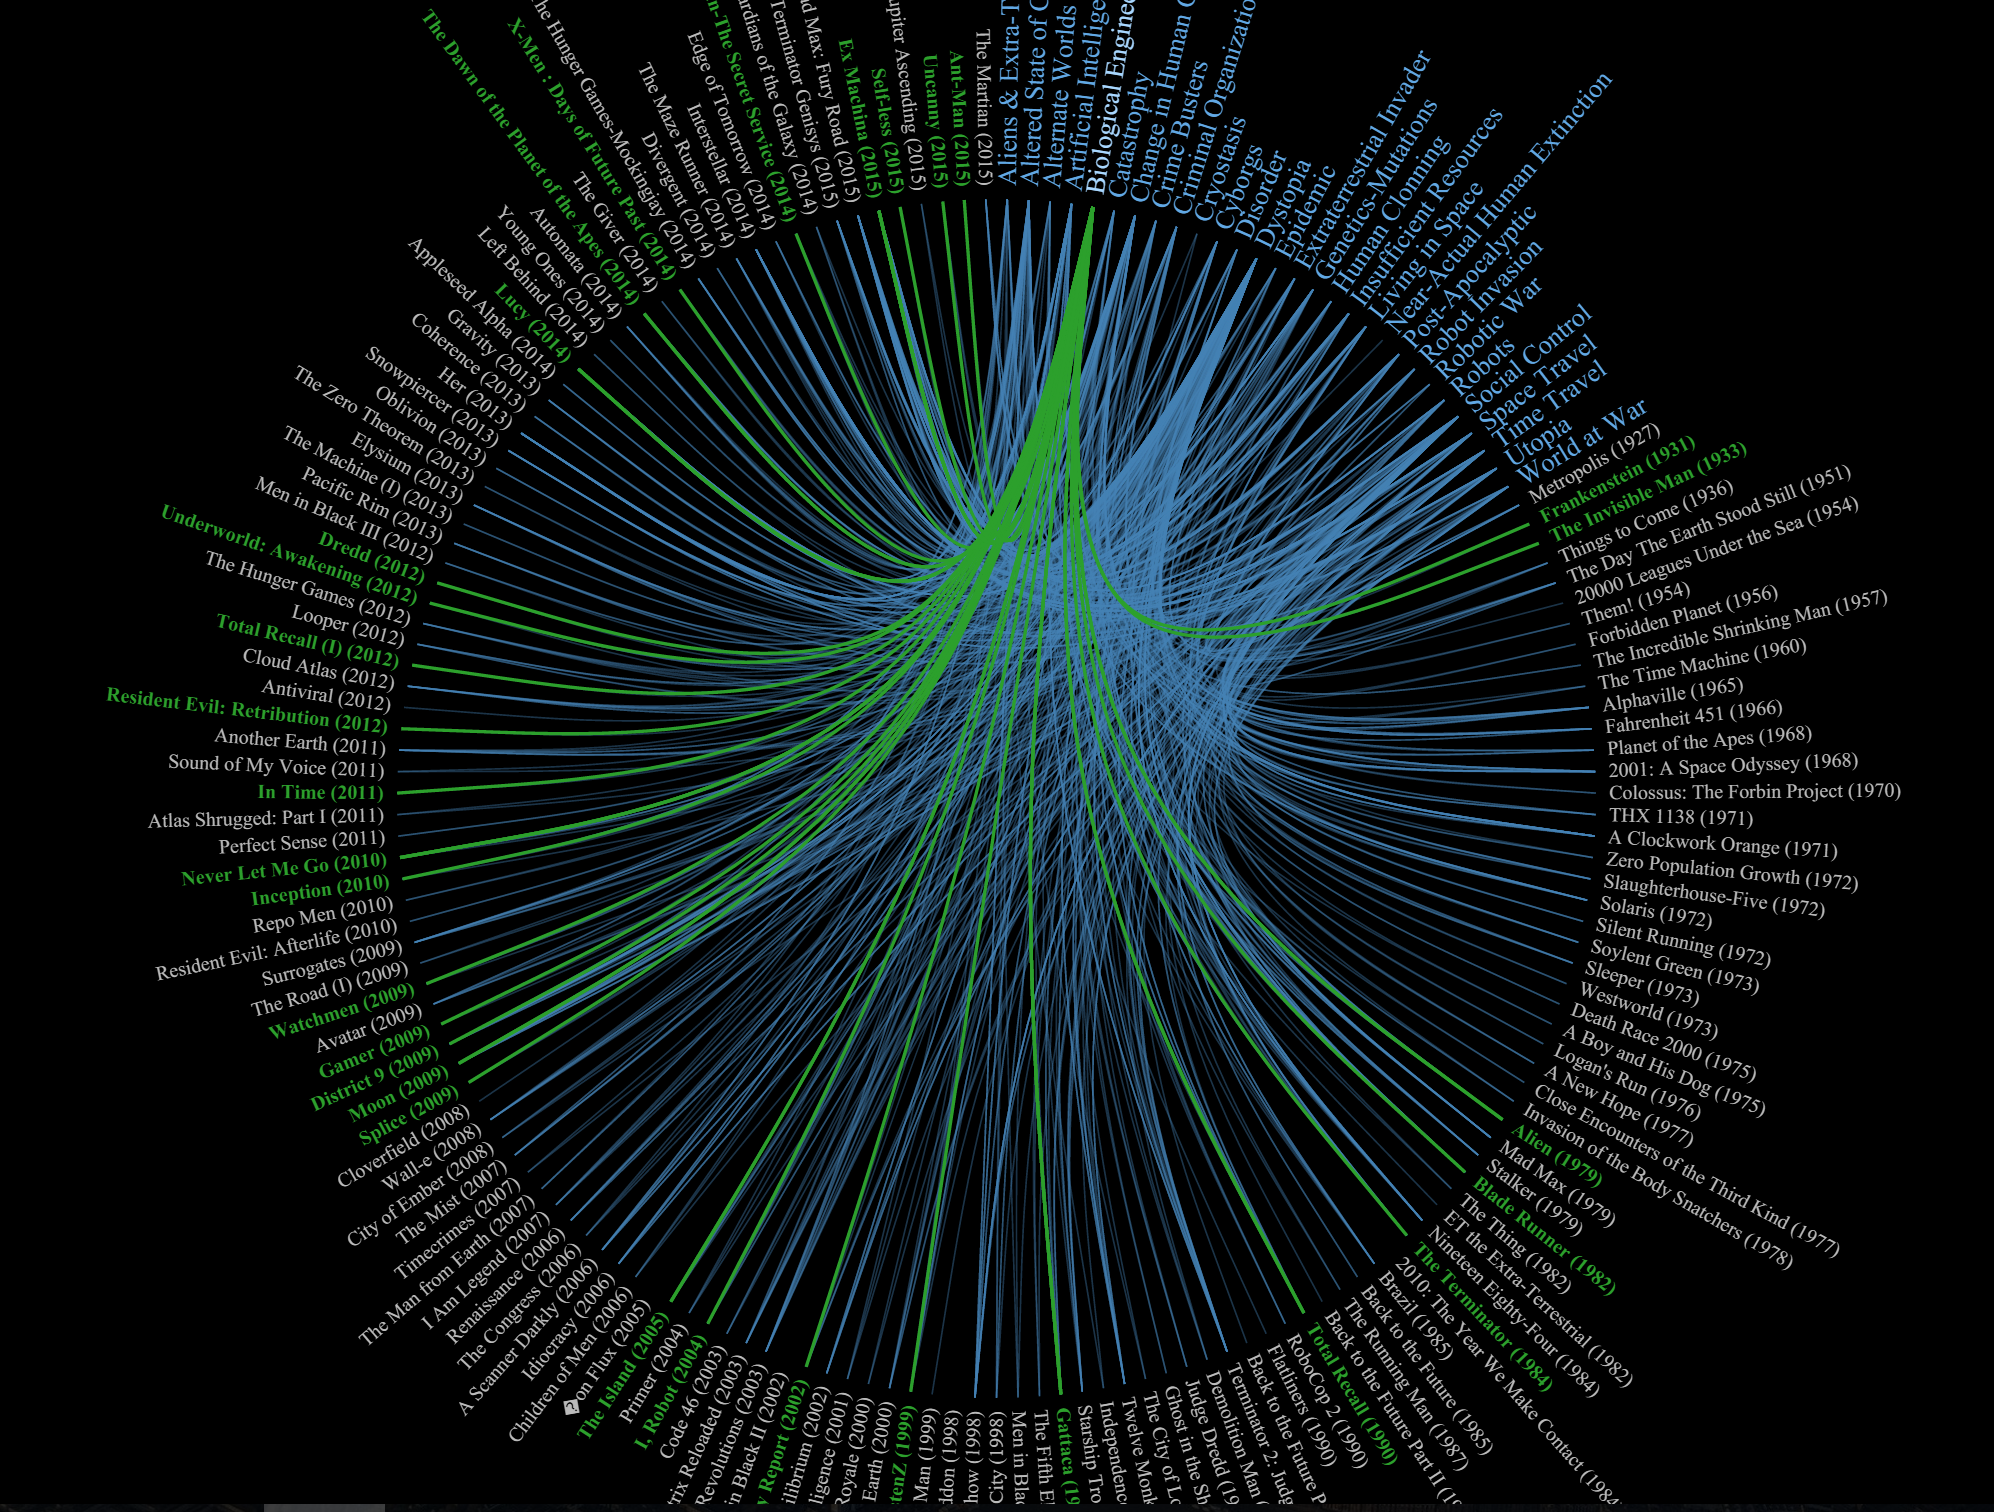
\includegraphics[width=\linewidth]{scifi.png}
	\centering
	\caption{Utopia-Dystopia: Use of Circos to describe links between large numbers of objects (sci-fi movies) ordered by a single variable (year).Sci-fi films ordered by year of release and themes displayed in a circle. Upon mousing over a topic films related to that topic are highlighted, or upon mousing over a film all topics in the film are highlighted. Allows patterns to be easily displayed such as biological engineering becoming an in vogue theme after 2009. Source: http://selcukartut.com/ \cite{scifi}}
	\label{fig:scifi}
\end{figure} 

Upon mousing over a profession 7 links are shown: The top 5 weighted heterosexual pairings, 1 male-male and 1 female-female non-weighted pairing. The use of similar colours and mixture of weighted and non-weighted links is confusing and hides a lot of the information about the true distribution. 


\begin{figure*}[htbp]
\centering
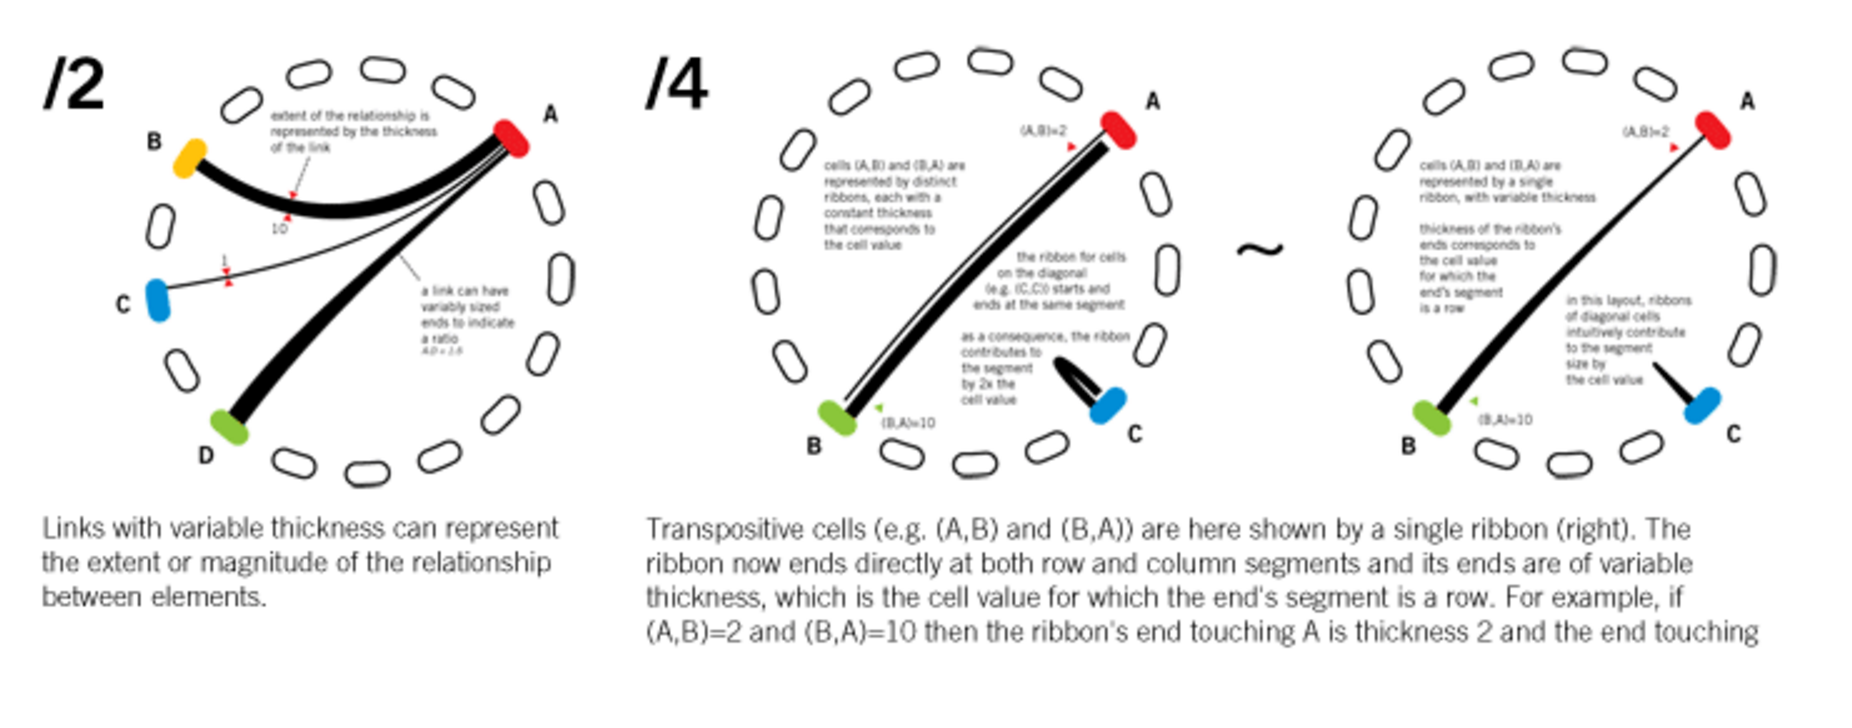
\includegraphics[width=\linewidth]{circos.png}
\caption{Methods for additional features encoded into Circos. /2 describes use of thickness to show weightings or distribution. /4 how self linking and reciprocal relationships can be described. 
source: Circos documentation /cite{circosimage}}
\label{fig:circos}
\end{figure*}

Showing the top percentage of marriages instead of a fixed number of links helps clarify distribution differences, avoid clutter by making ones beyond the 5th grey-scale. The male-male and female-female relationships should be more distinctly coloured, have more links shown and perhaps be shown separately so information about their distributions is clear.  

It appears the data hasn't been normalised, resulting in teachers, secretaries and nurses appearing very almost every selection, normalising the data would allow viewers to find more nuanced correlations. 

This visualisation embedded in an article, which points to specific examples. These points could be slightly highlighted to attract users attention following a Martini glass narrative structure\cite{narrative}.  

The narrative of this visualisation is to give the user the ability to explore the data but few tools are given to the user to do this. A Circos visualisation can encode this clearer (fig:\ref{fig:scifi}), without having to scroll and allow patterns to be spotted more easily\cite{circoscite}. Additional information can also be encoded with this method such as male:female ratio of marriages (fig:\ref{fig:circos}), allowing more levels of detail to be revealed one of Tufte's design principals \cite{tufte}.  



\section{Florida Gun Deaths\cite{floridagun}}
This is the now infamous graph of firearms murders in Florida following the introduction of a "Stand your ground" legislation. It was produced by Reuters to support a claim that the legislation had increased violence in the area. 

\begin{figure}[htbp]
	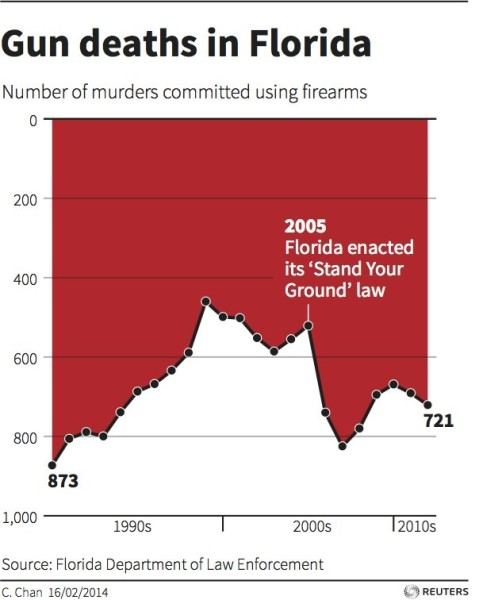
\includegraphics[width=\linewidth]{floridagun.jpg}
	\centering
	\caption{Number of murders committed using firearms in Florida since the 1990s published by reuters \ref{fig:floridagun}. Poor use of whitespace, caption and axis label placement confuses the viewer about inverted y axis.}
	\label{fig:floridagun}
\end{figure}

The source of confusion here is the inverted y axis, upon reflection it is clear the main reason for this design choice was to convey the imagery of blood. Aesthetic choices like this can add a lot to a graph intended for media consumption but only where they don't detract from the message \cite{sexy}.

The author Christine Chan was inspired by another Reuters graphic which used this technique successfully\cite{iraqdeaths}. The key differences here are that the Iraq visualisation has its Y axis at the top, uses the white-space for other charts, has annotations in the white-space and uses a bar chart instead of line chart which much clearer represents the dripping blood imagery. 

The title is confusing because the plot shows gun related murders but the title is about gun deaths. The plot therefore says nothing about how gun deaths has changed. In addition to this the graph would benefit from moving the numerical annotations to the area of interest and showing a US average in greyscale for comparison, this helps the design support the analysis. 
\begin{figure}[htbp]
	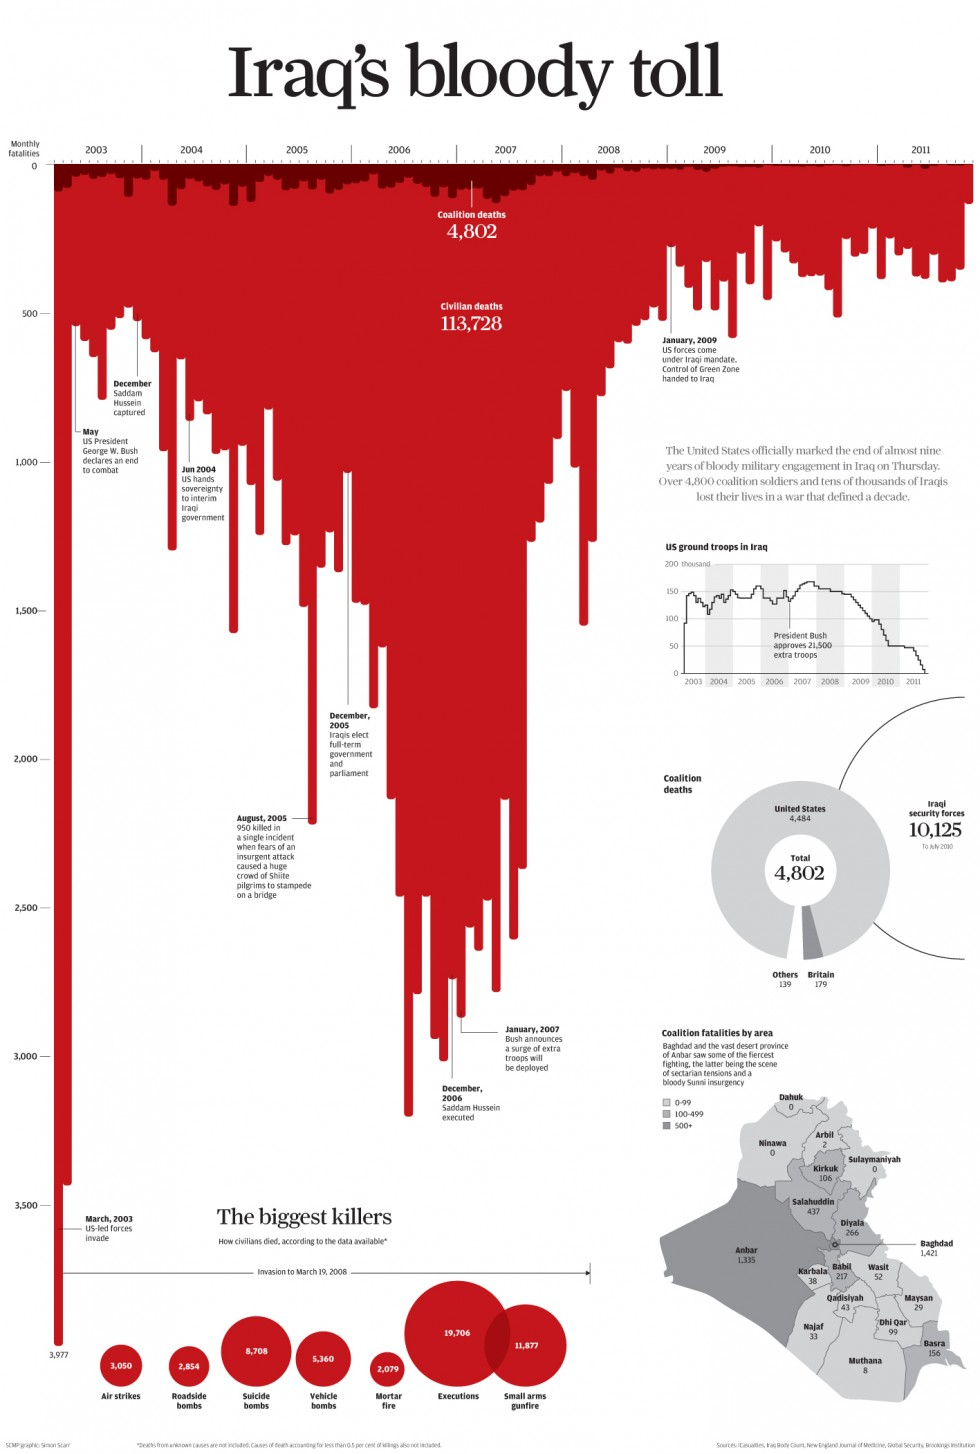
\includegraphics[width=0.5\textwidth]{iraqdeaths.jpg}
	\centering
	\caption{Iraq death toll visualisation from the South Cina Post. Uses whitespace to clearly show inverted y axis. Served as inspiration for figure \ref{fig:floridagun}. \cite{iraqdeaths}}
	\label{fig:iraqdeaths}
\end{figure} 

\section{Conclusion}
To conclude changes to visualisation conventions such are chart types or inverting axes can add to the overall image but there are caveats: Firstly there must be a clear reason for deviating and it not cloud the data (Bloomberg). Secondly the entire visualisation must support the design choice to clearly communicate it to the viewer and break their prior expectations. In such cases the invoking of imagery can actually add to reader comprehension of the data (xkcd). 

\small
\bibliographystyle{abbrv}
\bibliography{sigproc}

\end{document}
